\documentclass[a4paper]{article}
\usepackage{amsfonts}
\usepackage{amsmath}
\usepackage{amssymb}
\usepackage{graphicx}     

\newcommand{\Bgtan}{\operatorname{Bgtan}}
\newcommand{\Bgsin}{\operatorname{Bgsin}}

\begin{document}
  
\noindent \large Auteur: Zaky Souai \\
\noindent \large Studierichting:  Informatica\\
\noindent \large Oefeningenreeks 5D nr. 1.15\\

\bigskip

\normalsize

$5^x>0 \Rightarrow f(x)>0$\\

Dus de oppervlakte tussen de grafiek en de $X$-as is:

$A=\displaystyle\int_0^1 5^x dx$\\

$A=\left[\dfrac{5^x}{\ln 5}\right]_0^1$\\

$=\dfrac{5^1}{\ln 5}-\dfrac{5^0}{\ln 5}$\\

$=\dfrac{5}{\ln 5}-\dfrac{1}{\ln 5}$\\

$=\dfrac{4}{\ln 5}$\\

\begin{figure}[h]
\centering
    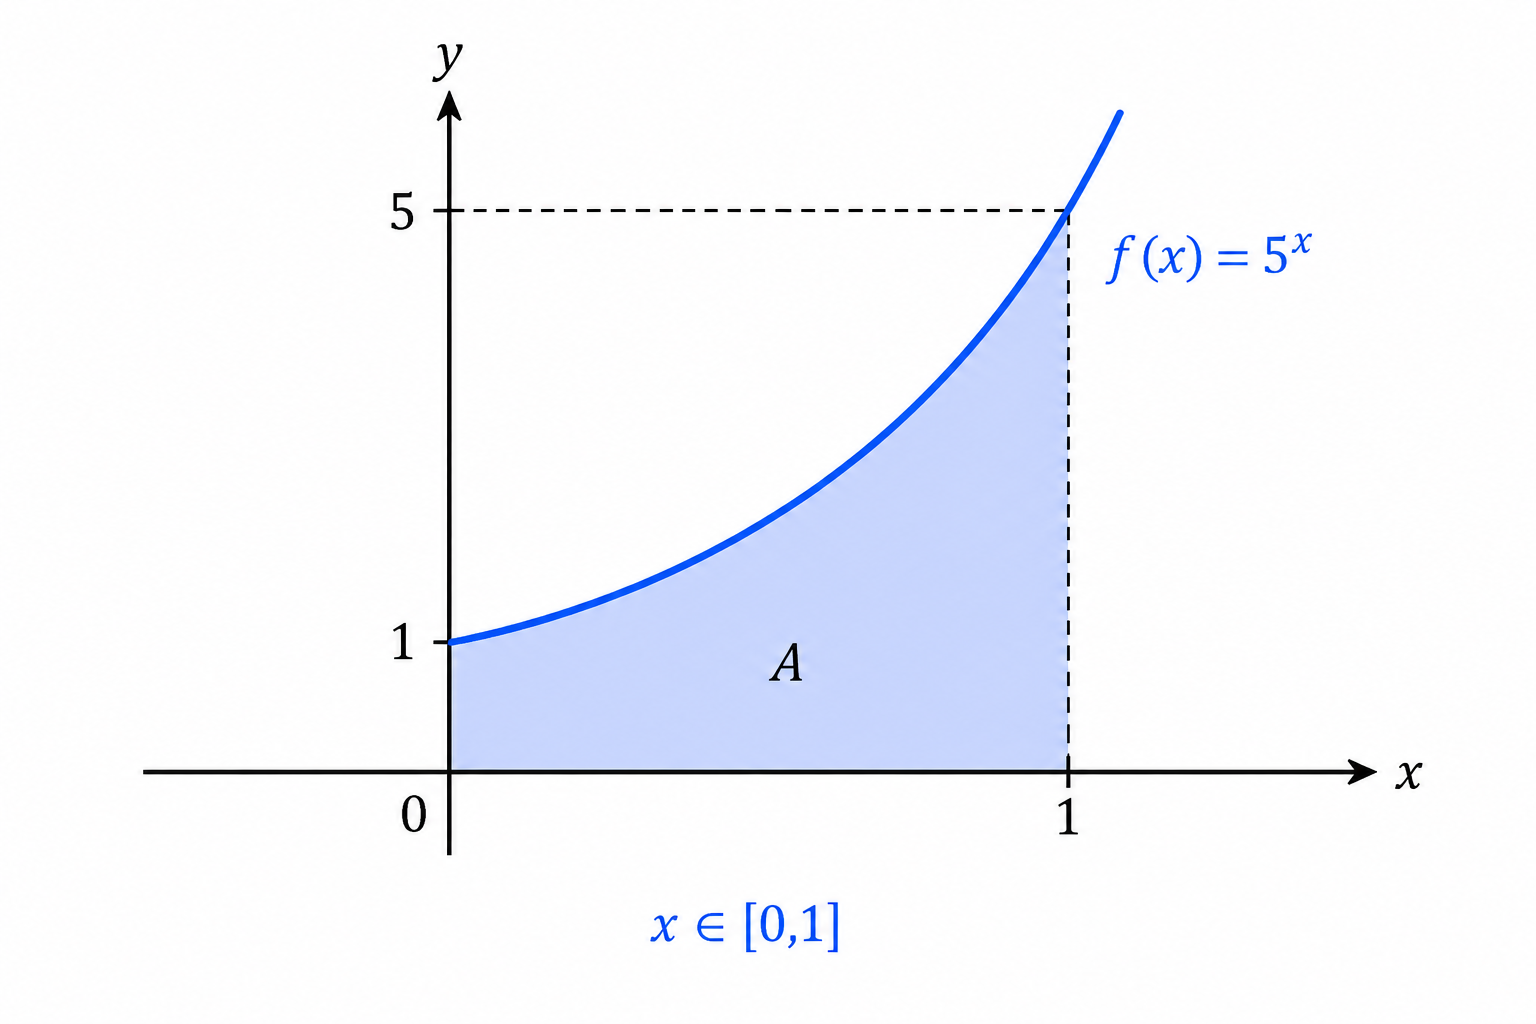
\includegraphics[width=\linewidth]{5D-1.15-zaky.souai.INF.png}\\
\end{figure}

\begin{thebibliography}{999}
%\bibitem{a} Referentie
\end{thebibliography}
\end{document}